\section{Patterns 4 - State patterns}

\subsection{Fokuspunkter}

\begin{itemize}
	\item Redegør for, hvad et software design pattern er.
	%\item Redegør for de forskellige måder at implementere en state machine på.
	\item Redegør for strukturen i GoF State Pattern.
	\item Sammenlign  switch/case-implementering med GoF State.
	\item Redegør for fordele og ulemper ved anvendelsen af GoF State.
	\item Redegør for, hvordan et UML (SysML) state machine diagram mapper til GoF State.
\end{itemize}

\subsection{Hvad er et Software pattern?}

\derp

\subsection{Redegør for strukturen i et state pattern}
Et state pattern er et behavioral pattern, og er en måde at implementere en state machine på.

State mønstret definerer en måde hvorpå vi kan ændre et objekts opførsel eftersom dens interne state ændres (run-time).
State mønstret giver mulighed for at implementere store forskelle i opførslen uden brug af masser af Switches of if sætninger.

\begin{figure}[h]
\centering
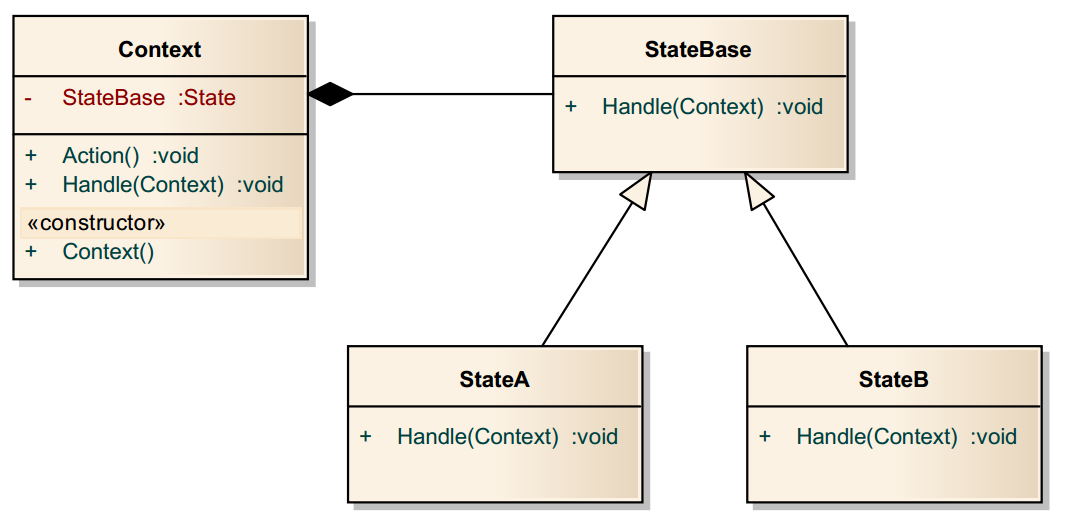
\includegraphics[width=0.8\linewidth]{figs/newstate/statepattern_simple}
\caption{UML for et GoF state pattern}
\label{fig:gofState}
\end{figure}

\begin{enumerate}
	\item Context klassen
	\begin{itemize}
		\item Definerer et interface der bruges af klienter.
		\item Indeholder en instans af en ConreteState subclass, der kan definere en Current State.
		\item Indeholder Actions.
	\end{itemize}
	\item StateBase klassen
	\begin{itemize}
		\item Et interface til indkapsling af ConcreteStates adfærd
		\item Indeholder virtuelle handles.
		\item 
	\end{itemize}
	\item Concrete State
	\begin{itemize}
		\item  Hver ConcreteState implementerer den adfærd der associeres til i Context klassen (handle til hver action).
	\end{itemize}
\end{enumerate}

\subsubsection{Kodeeksempel}

Dette er et kodeekspempel på en state machine der kan toggle dens state.

\begin{lstlisting}[caption=StateBase klassen,
morekeywords={abstract, Context}]
abstract class State
{
	public abstract void Handle(Context context);
}
\end{lstlisting}

Som det ses på klassen StateBase implementering, har den blot en abstrakt metode der tager mod en Context

\begin{lstlisting}[caption=ConcreteStateA klassen - Switcher til State B,
morekeywords={abstract, Context}]
class ConcreteStateA : State
{
	public override void Handle(Context context)
	{
		context.State = new ConcreteStateB;
	}
}
\end{lstlisting}

\begin{lstlisting}[caption=StateBase klassen - Switcher til state A,
morekeywords={abstract, Context}]
class ConcreteStateB : State
{
	public override void Handle(Context context)
	{
		context.State = new ConcreteStateA;
	}
}
\end{lstlisting}


\begin{minipage}{\linewidth}
\begin{lstlisting}[caption=Context klassen - Bruges i main() til at kalde Request(),
morekeywords={abstract, Context}]
class Context
{
	private State _state;
	
	// Constructor
	public Context(State state)
	{
		this.State = state;
	}
	
	// Gets or sets the state
	public State State
	{
		get { return _state; }
		set
		{
			_state = value;
			Console.WriteLine("State: " + _state.GetType().Name);
		}
	}
	
	public void Request()
	{
		_state.Handle(this);
	}
}
\end{lstlisting}
\end{minipage}

I lærebogen erklæres alle states static inde i contexten idet der således ikke skal laves en ny, hver gang der skiftes state... Smart.

\paragraph{State vs. Strategy.}
Ser man på UML'en for et State Pattern, ligner det jo et strategy pattern. I et State  pattern eksisterer der dog et constraint idet hver ConcreteState klasse skal bruge en reference til en Context (den vælger og invoker contextens metoder igennem denne reference). Dette constraint eksisterer ikke i et strategy pattern:

\begin{lstlisting}[caption=Klients brug af strategy pattern,
morekeywords={abstract, Context}]
IStrategy myStrategy = new s1();
myStrategy.StragetyFunction();

myStrategy = new s2();
myStrategy.StragetyFunction();
\end{lstlisting}

Ortogonale og nestede states gennemgås i afsnittet om UML mapping.

\subsection{Sammenlign switch/case-implementering med GoF State.}

\subsubsection{Switch case implementering af STM}
\begin{itemize}
	\item En switch case implementering af en STM er det simple udgave.
	\item Koden bliver meget hurtig uoverskulig.
	\item Den er sværere at teste (Dårligt separeret)
	\item Sværere at vedligereholde.
\end{itemize}

\subsubsection{GoF State implementering af STM}
\begin{itemize}
	\item Grundig implmentering af STM.
	\item Alle states er inddelt i subclasser af en State baseklasse.
	\item Derfor let at teste.
	\item Og lettere at vedligeholde.
\end{itemize}

\subsection{Redegør for fordele og ulemper ved anvendelsen af GoF State.}

\subsubsection{Fordele}
\begin{itemize}
	\item Let at teste - de mange klasser gør det enkelt at afgrænse tests.
	\item Let at udvide - Skalerer nemt ved udvidelser af både states og transitions.
	\item Kan lettere håndtere Nested States-
	\item Forholdsvis simpelt at implementere Ortogonale states.
\end{itemize}

\subsubsection{Ulemper}
\begin{itemize}
	\item Class Explosion - ved et simpelt STM skal der oprettes mange klasser for meget simpel logik, der vil derfor være en nedre grænse for hvornår man vil implementere dette.
	\item Memory - Flere klasser betyder mere memory allokering.
	\item Readability - i mere komplekse programmer vil koden blive svær at overskue, men er dog stadig væsentligt nemmere end alternativerne.
\end{itemize}

\todo{uløst problem med OnExit() Andreas/Denned??}

\subsection{Redegør for, hvordan et UML (SysML) state machine diagram mapper til GoF State}
\subsubsection{Simpel UML}

Et simpelt STM UML Diagram:

\begin{figure}[H]
	\centering
	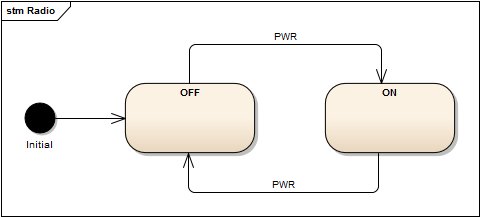
\includegraphics[width=0.8\linewidth]{figs/state/Radio_STM_Simpel}
	\caption{Et UML State Machine Diagram}
	\label{fig:UMLState}
\end{figure}

Et tilsvarende GoF State Pattern klassediagram for en radioen:

\begin{figure}[H]
	\centering
	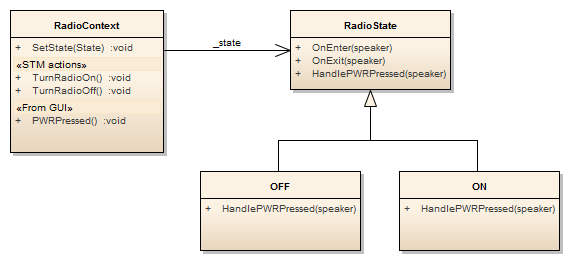
\includegraphics[width=0.8\linewidth]{figs/state/Radio_StatePattern}
	\caption{Et UML Klassediagram for STD}
	\label{fig:UMLclassState}
\end{figure}

\subsubsection{Nestede States}

Et STM UML diagram med nested states:

\begin{figure}[H]
	\centering
	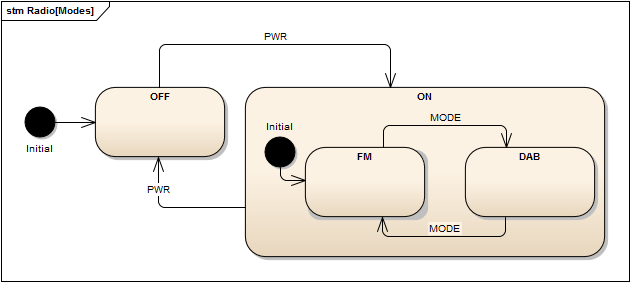
\includegraphics[width=0.9\linewidth]{figs/state/Radio[Modes]_STM}
	\caption{Et UML State Machine Diagram for Nested states}
	\label{fig:UMLNestedState}
\end{figure}

Et tilsvarende GoF State Pattern klassediagram med nested states:

\begin{figure}[H]
	\centering
	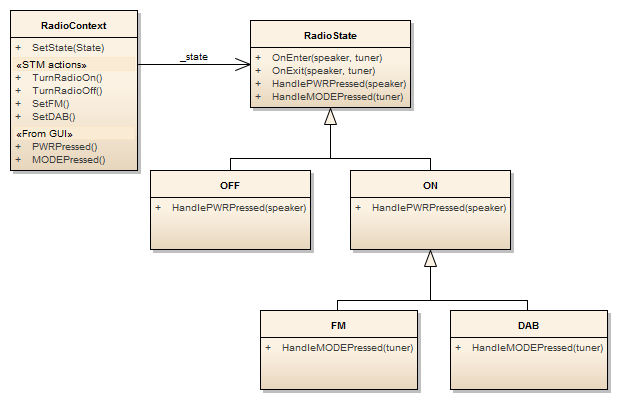
\includegraphics[width=0.9\linewidth]{figs/state/RadioNeted_SP}
	\caption{Et UML Klassediagram for Nested states}
	\label{fig:UMLClassNestedState}
\end{figure}

Vi kan her se i det tilsvarende State pattern, at den blot har to state klasser der hedder “FM” og “DAB” der nedarver fra ON klassen som set tidligere. og dertil mindre ændringer i Context klassens funktioner. %\todo{bryder vi ikke ISP her? Vi bryder i hvert fald LSP.} - LSP er nok ikke relevant i den sammenhæng...

\subsubsection{Ortogonale States}
Et STM UML diagram med ortogonale states på figur~\ref{fig:umlOrtogonalState}:

\begin{figure}[H]
	\centering
	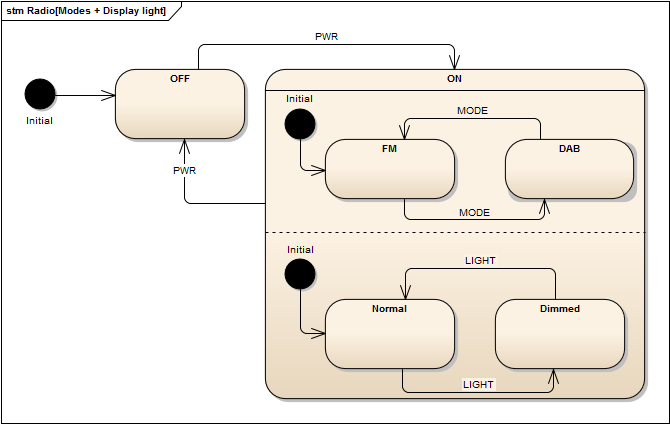
\includegraphics[width=\linewidth]{figs/state/RadioModesDisplayLight}
	\caption{Et UML State Machine Diagram for ortogonale states}
	\label{fig:umlOrtogonalState}
\end{figure}

Et tilsvarende GoF State Pattern klassediagram med ortogonale states:

\begin{figure}[H]
	\centering
	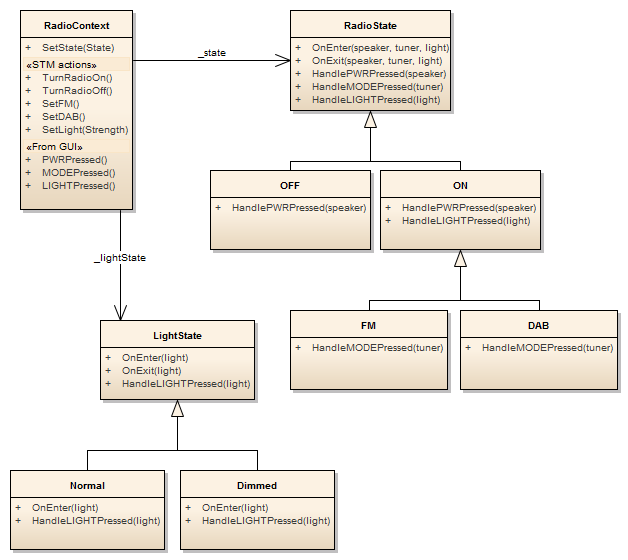
\includegraphics[width=\linewidth]{figs/state/RadioOrthogonal_SP}
	\caption{Et UML Klassediagram for Nested states}
	\label{fig:UMLClassOrtogonalState}
\end{figure}

Læg her mærke til at Ortogonale statemachines, kræver blot en ekstra “superstate” med dertilhørende substates, denne superstate bliver en reference i contexten som dermed gør at de to forskellige superstates kan tilgå hinanden.

